\documentclass[../differential_geometry.tex]{subfiles}
\begin{document}
\section{Aula 08 - de Fevereiro, 2026}
\subsection{Motivações}
\begin{itemize}
	\item Definição de uma Superfície;
	\item Gráfico de uma Função;
	\item Pré-imagem de um Valor Regular de uma Função.
\end{itemize}
\subsection{Um Exemplo do Teorema da Função Implícita}
Vamos considerar a função \(f:\mathbb{R}^{3}\rightarrow \mathbb{R}^{2}\) dada por
\[
	f(x, y, z)=(y+x^{2}, z-x^{3}).
\]
Aqui, temos
\[
	f(0,0,0)=0 \quad\&\quad J_{(x, y, z)}f = \begin{pmatrix}
		2x      & 1 & 0 \\
		-3x^{2} & 0 & 1
	\end{pmatrix}
\],
ou seja, se \((a, b)=(0, (0,0))\in \mathbb{R}\times \mathbb{R}^{2}=\mathbb{R}^{3},\) então
\[
	\begin{pmatrix}
		\frac{\partial^{}f^{1}}{\partial y^{}} & \frac{\partial^{}f^{1}}{\partial z^{}} \\
		\frac{\partial^{}f^{2}}{\partial y^{}} & \frac{\partial^{}f^{2}}{\partial z^{}}
	\end{pmatrix} = \begin{pmatrix}
		1 & 0 \\
		0 & 1
	\end{pmatrix}.
\]
Logo, pelo \hyperlink{implicit_function}{\textit{Teorema da Função Implícita}}, existem abertos V de \(\mathbb{R}\) e W de \(\mathbb{R}^{2}\), e uma função \(g:V\rightarrow W\), tais que
\[
	(x, y, z)\in V\times W:\; f(x,y,z)=0 \Longleftrightarrow (y, z)=g(x).
\]
Esse exemplo é particularmente legal, porque ele permite obter a expressão explícita de g! De fato,
\begin{align*}
	f(x,y,z)=0 & \Longleftrightarrow y+x^{2}=0 \quad\&\quad z-x^{3}=0 \\
	           & \Longleftrightarrow \left\{\begin{array}{ll}
		                                        y=-x^{2} \\
		                                        z=x^{3}
	                                        \end{array}\right.        \\
	           & g(x)=(-x^{2}, x^{3})
\end{align*}
\subsection{Superfícies e Funções}
Intuitivamente, uma curva é uma deformação de um segmento de reta; assim, também é intuitivo pensarmos nas superfícies como, possivelmente, a deformação local de um aberto de \(\mathbb{R}^{2}.\)
\begin{figure}[H]
	\begin{center}
		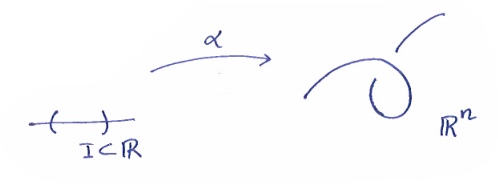
\includegraphics[height=0.5\textheight, width=0.5\textwidth, keepaspectratio]{./Images/line_to_curve_08.png}
		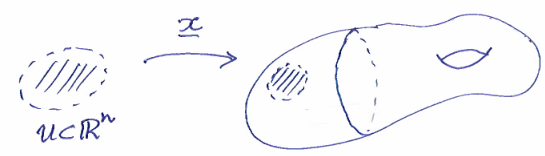
\includegraphics[height=0.5\textheight, width=0.5\textwidth, keepaspectratio]{./Images/open_to_surface_08.png}
	\end{center}
	\caption{correção: \(U\subseteq \mathbb{R}^{2}\).}
\end{figure}
Porém, não queremos uma definição de superfícies que tenham certos problemas, especificamente as que possuem pontos de autointerseção ou \textit{singulares.}
\begin{figure}[H]
	\begin{center}
		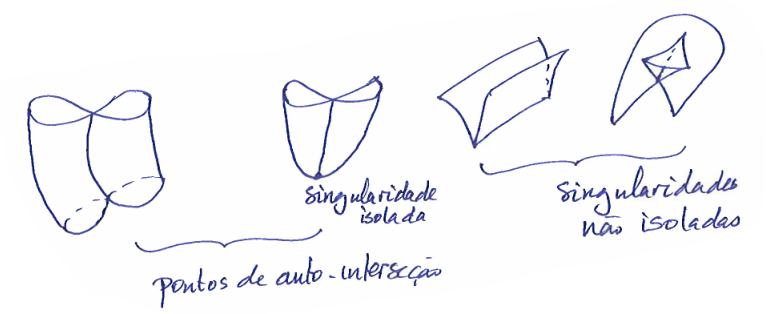
\includegraphics[height=0.7\textheight, width=0.7\textwidth, keepaspectratio]{./Images/singularities_surfaces_08.png}
	\end{center}
	\caption{superfícies com pontos de singularidades isoladas, não isoladas e pontos de autointerseção}
\end{figure}
\begin{def*}
	Um subconjunto \(S\subseteq \mathbb{R}^{3}\) é uma \textbf{superfície regular} se, em cada ponto p de S, existir um aberto V de \(\mathbb{R}^{3}\) contendo p e uma aplicação \(\underline{x}:U\subseteq \mathbb{R}^{2}\rightarrow V\cap S\), onde U é um aberto de \(\mathbb{R}^{2}\), tal que:
	\begin{itemize}
		\item[1)] A aplicação \(\underline{x}\) é suave: se \(\underline{x}(u, v)=(x(u, v), y(u, v), z(u,v)\), então\linebreak \(x(u, v),\; y(u, v)\) e \(z(u, v)\) são funções suaves (lida com as singularidades isoladas);
		\item[2)] A aplicação \(\underline{x}:U\rightarrow V\cap S\) é um homeomorfismo, ou seja, tem uma inversa \(\underline{x}^{-1}:V\cap S\rightarrow U\) e ela é contínua (lida com as autointerseções);
		\item[3)] As derivadas parciais \(\underline{x}_{u}=\partial_{u}x\) e \(\underline{x}_{v}=\partial_{v}x\) com respeito às variáveis u e v são linearmente independentes em todos os pontos (lida com o terceiro tipo de problema, as singularidades não isoladas).
	\end{itemize}
	Nestas condições, \(\underline{x}\) é chamada \textbf{parametrização local de S em p}, \(\underline{x}^{-1}\) é chamada \textbf{carta local de S em p}, e \(V\cap S\) é chamada \textbf{vizinhança de coordenada.} \(\square\)
\end{def*}
\begin{tcolorbox}[
		skin=enhanced,
		title=Observação,
		fonttitle=\bfseries,
		colframe=black,
		colbacktitle=cyan!75!white,
		colback=cyan!15,
		colbacklower=black,
		coltitle=black,
		drop fuzzy shadow,
		%drop large lifted shadow
	]
	Podemos usar (1), (2) e (3) para definir uma superfície em \(\mathbb{R}^{n},\; n > 3\).
\end{tcolorbox}
Temos duas proposições que são úteis na verificação de um subconjunto de \(\mathbb{R}^{3}\) ser ou não uma superfície.

\begin{prop*}
	Seja \(g:U\subseteq \mathbb{R}^{2}\rightarrow \mathbb{R}\) uma função suave, onde U é aberto. O gráfico da função g, definido por
	\[
		\Gamma (g)\coloneqq \{(u, v, g(u, v)):\; (u, v)\in U\}\subseteq \mathbb{R}^{3},
	\]
	é uma superfície de \(\mathbb{R}^{3}\).
\end{prop*}
\begin{proof*}
	Vamos definir a parametrização por
	\begin{align*}
		\underline{x}: & U\rightarrow\Gamma (g)\cap \mathbb{R}^{3} \\
		               & (u, v)\longmapsto (u, v, g(u, v)).
	\end{align*}
	Tomando \(V = \mathbb{R}^{3}\), temos a suavidade de \(\underline{x}\) e a bijetividade:
	\begin{align*}
		\underline{x}(u, v)= \underline{x}(u', v') & \Longleftrightarrow (u, v, g(u, v))=(u', v', g(u', v')) \\
		                                           & \Longleftrightarrow (u, v)=(u', v'),
	\end{align*}
	garantindo a existência da inversa \(\underline{x}^{-1}\), e a continuidade da mesma segue observando que \(\underline{x}^{-1}\) nada mais é do que a projeção \( \pi : \mathbb{R}^{3}\rightarrow \mathbb{R}^{2}\), restrita a S. (Vale lembrar que \( \pi (x, y, z)=(x,y)\) é contínua).

	Por fim, basta notar que as derivadas parciais são
	\[
		\underline{x}_{u}=(1,0, g_{u}(u, v)) \quad\&\quad \underline{x}_{v}=(0,1, g_{v}(u, v)),
	\]
	e portanto são linearmente independentes para todo par \((u, v)\in U\). \qedsymbol
\end{proof*}
\begin{tcolorbox}[
		skin=enhanced,
		title=Observação,
		fonttitle=\bfseries,
		colframe=black,
		colbacktitle=cyan!75!white,
		colback=cyan!15,
		colbacklower=black,
		coltitle=black,
		drop fuzzy shadow,
		%drop large lifted shadow
	]
	O resultado acima pode ser generalizado para dimensões maiores que 3: dada uma função \(g:U\subseteq \mathbb{R}^{2}\rightarrow \mathbb{R}^{n-2},\; n>3,\;\) suave, então o gráfico de g
	\[
		\Gamma (g)=\{((u, v), g^{1}(u, v), \dotsc , g^{n-2}(u, v)):\; (u, v)\in U\},
	\]
	é uma superfície em \(\mathbb{R}^{n}.\)
\end{tcolorbox}
\begin{example}[Paraboloide Elíptico]
	O paraboloide elíptico é uma superfície dada por
	\[
		g(u, v)=\frac{u^{2}}{a^{2}}+\frac{v^{2}}{b^{2}}.
	\]
	\begin{figure}[H]
		\begin{center}
			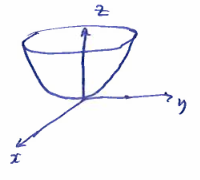
\includegraphics[height=0.4\textheight, width=0.4\textwidth, keepaspectratio]{./Images/parabolloid_08.png}
		\end{center}
		\caption{paraboloide elíptico em \(\mathbb{R}^{3}\)}
	\end{figure}
\end{example}
\begin{example}[Paraboloide Hiperbólico]
	O paraboloide hiperbólico é uma superfície em \(\mathbb{R}^{3}\) dado por
	\[
		g(u, v)=\frac{u^{2}}{a^{2}}-\frac{v^{2}}{b^{2}}.
	\]
	\begin{figure}[H]
		\begin{center}
			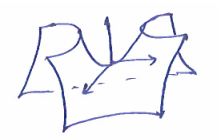
\includegraphics[height=0.35\textheight, width=0.35\textwidth, keepaspectratio]{./Images/hyperbolic_parabolloid_08.png}
		\end{center}
	\end{figure}
\end{example}
\begin{example}[Esfera de raio r]
	Seja
	\[
		S(r)=\{(x,y,z)\in \mathbb{R}^{3}:\; x^{2}+y^{2}+z^{2}=r^{2}\},
	\]
	onde \(r\geq 0\), resultando na \textbf{esfera de raio r}; então, ela é uma superfície!
	\begin{figure}[H]
		\begin{center}
			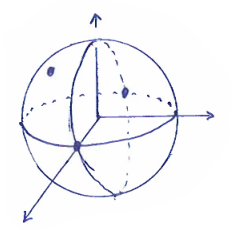
\includegraphics[height=0.4\textheight, width=0.4\textwidth, keepaspectratio]{./Images/sphere_08.png}
		\end{center}
	\end{figure}

	De fato, seja \(p=(a, b, c)\) um ponto na esfera de raio r que não pertença ao equador, ou seja, não pertence à circunferência \((a, b, 0)\). Temos, então,
	\begin{align*}
		(x, y, z)\in S(r) & \Longleftrightarrow x^{2}+y^{2}+z^{2}=r^{2}                                                                                               \\
		                  & \Longleftrightarrow z = \sqrt[]{r^{2}-x^{2}-y^{2}}\eqqcolon g_{1}(x, y) \text{ ou } z = -\sqrt[]{r^{2}-x^{2}-y^{2}}\eqqcolon g_{2}(x, y).
	\end{align*}
	Sendo assim, considere as aplicações definidas acima, dadas por \(g_{i}:B((0,0), r)\subseteq \mathbb{R}^{2}\rightarrow \mathbb{R},\; i=1,2\); estas funções são suaves, tal que, pela proposição provada acima, seus gráficos são superfícies em \(\mathbb{R}^{3}\)! Neste caso, vale
	\[
		\Gamma (g_{1})\cup \Gamma (g_{2})=S(r)\setminus{\text{Equador}}.
	\]
	Porém, e se olharmos para um ponto no equador?

	Ora, tomemos \(p=(a, b, 0)\) um ponto no equador tal que \(a\neq 0\) ou \(b\neq 0\). Primeiramente, vamos supor que a segunda situação ocorre: como \(b\neq 0\), então p pertence ao gráfico da função
	\[
		g_{3}(x, z)=\sqrt[]{r^{2}-x^{2}-z^{2}},
	\]
	ou da função
	\[
		g_{4}(x, z)=-\sqrt[]{r^{2}-x^{2}-z^{2}}.
	\]

	Por outro lado, se \(a\neq 0\), tal que \(p=(\pm r, 0, 0)\), então ele pertence ao gráfico da função
	\[
		g_{5}(y, z)=\sqrt[]{r^{2}-y^{2}-z^{2}},
	\]
	ou da função
	\[
		g_{6}(y, z)=-\sqrt[]{r^{2}-y^{2}-z^{2}}.
	\]

	Portanto, as funções \(g_{i}:B((0,0), r)\subseteq \mathbb{R}^{2}\rightarrow \mathbb{R},\; i=3,4,5,6\), são todas suaves, concluindo justamente que seus gráficos são superfícies em \(\mathbb{R}^{3}.\)
\end{example}

\end{document}

